\chapter{Algorismes d'escombrat de línies}

\index{línia d'escombrat}

Molts problemes geomètrics es poden resoldre fent servir algorismes de
\key{línia d'escombrat} (\emph{sweep line}). La idea en aquests
algorismes és representar una instància del problema com un conjunt
d'esdeveniments que es corresponen amb punts del pla. Els
esdeveniments es processen en ordre creixent segons les seves
coordenades $x$ o $y$.

A tall d'exemple, considereu el problema següent: una empresa té $n$
empleats, i sabem per a cada empleat a quina hora ha arribat i quina
hora ha sortit un dia donat. La nostra tasca és calcular el nombre
màxim d'empleats que hi havia a l'oficina alhora.

El problema es pot resoldre modelant la situació de manera que a cada
empleat se li assignin dos esdeveniments que corresponen als seus
horaris d'arribada i sortida. Després d'ordenar els esdeveniments, els
repassem i fem un seguiment del nombre de persones a l'oficina. Per
exemple, la taula
\begin{center}
\begin{tabular}{ccc}
persona & temps d'arribada & temps de sortida \\
\hline
John & 10 & 15 \\
Maria & 6 & 12 \\
Peter & 14 & 16 \\
Lisa & 5 & 13 \\
\end{tabular}
\end{center}
correspon als següents esdeveniments:
\begin{center}
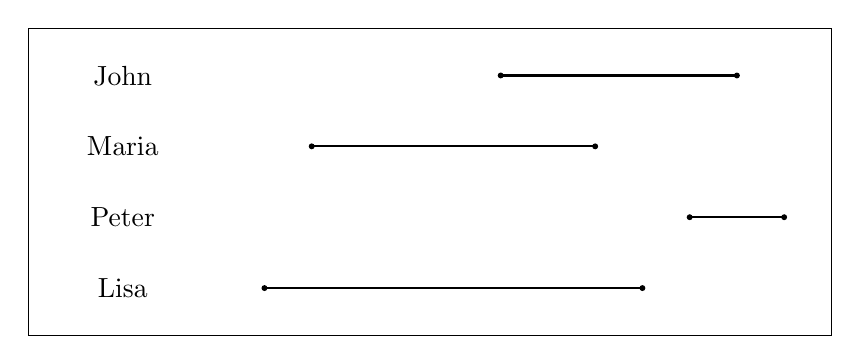
\begin{tikzpicture}[scale=0.6]
\draw (0,0) rectangle (17,-6.5);
\path[draw,thick,-] (10,-1) -- (15,-1);
\path[draw,thick,-] (6,-2.5) -- (12,-2.5);
\path[draw,thick,-] (14,-4) -- (16,-4);
\path[draw,thick,-] (5,-5.5) -- (13,-5.5);

\draw[fill] (10,-1) circle [radius=0.05];
\draw[fill] (15,-1) circle [radius=0.05];
\draw[fill] (6,-2.5) circle [radius=0.05];
\draw[fill] (12,-2.5) circle [radius=0.05];
\draw[fill] (14,-4) circle [radius=0.05];
\draw[fill] (16,-4) circle [radius=0.05];
\draw[fill] (5,-5.5) circle [radius=0.05];
\draw[fill] (13,-5.5) circle [radius=0.05];

\node at (2,-1) {John};
\node at (2,-2.5) {Maria};
\node at (2,-4) {Peter};
\node at (2,-5.5) {Lisa};
\end{tikzpicture}
\end{center}
Repassem els esdeveniments d'esquerra a dreta i mantenim un
comptador. Sempre quan arriba una persona, augmentem el valor del
comptador en un, i quan una persona marxa, reduïm el valor del
comptador en un. La resposta al problema és el valor màxim del
comptador durant l'algorisme.

En aquest exemple els esdeveniments es processen de la següent manera:
\begin{center}
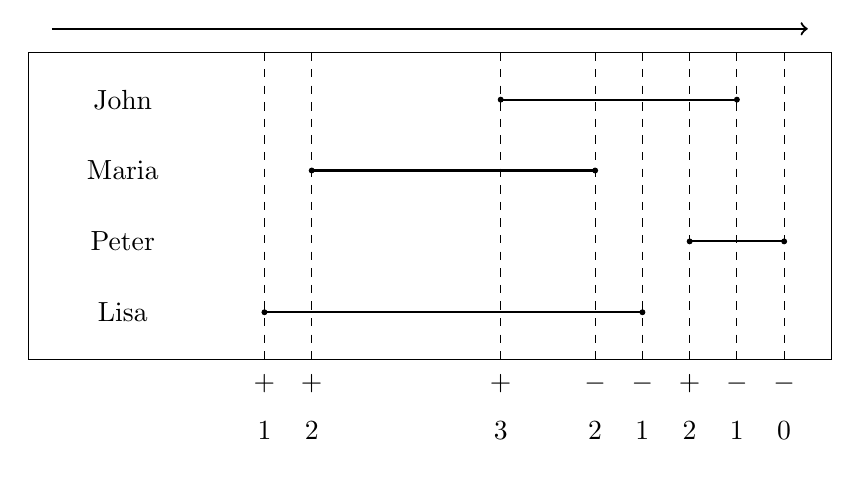
\begin{tikzpicture}[scale=0.6]
\path[draw,thick,->] (0.5,0.5) -- (16.5,0.5);
\draw (0,0) rectangle (17,-6.5);
\path[draw,thick,-] (10,-1) -- (15,-1);
\path[draw,thick,-] (6,-2.5) -- (12,-2.5);
\path[draw,thick,-] (14,-4) -- (16,-4);
\path[draw,thick,-] (5,-5.5) -- (13,-5.5);

\draw[fill] (10,-1) circle [radius=0.05];
\draw[fill] (15,-1) circle [radius=0.05];
\draw[fill] (6,-2.5) circle [radius=0.05];
\draw[fill] (12,-2.5) circle [radius=0.05];
\draw[fill] (14,-4) circle [radius=0.05];
\draw[fill] (16,-4) circle [radius=0.05];
\draw[fill] (5,-5.5) circle [radius=0.05];
\draw[fill] (13,-5.5) circle [radius=0.05];

\node at (2,-1) {John};
\node at (2,-2.5) {Maria};
\node at (2,-4) {Peter};
\node at (2,-5.5) {Lisa};

\path[draw,dashed] (10,0)--(10,-6.5);
\path[draw,dashed] (15,0)--(15,-6.5);
\path[draw,dashed] (6,0)--(6,-6.5);
\path[draw,dashed] (12,0)--(12,-6.5);
\path[draw,dashed] (14,0)--(14,-6.5);
\path[draw,dashed] (16,0)--(16,-6.5);
\path[draw,dashed] (5,0)--(5,-6.5);
\path[draw,dashed] (13,0)--(13,-6.5);

\node at (10,-7) {$+$};
\node at (15,-7) {$-$};
\node at (6,-7) {$+$};
\node at (12,-7) {$-$};
\node at (14,-7) {$+$};
\node at (16,-7) {$-$};
\node at (5,-7) {$+$};
\node at (13,-7) {$-$};

\node at (10,-8) {$3$};
\node at (15,-8) {$1$};
\node at (6,-8) {$2$};
\node at (12,-8) {$2$};
\node at (14,-8) {$2$};
\node at (16,-8) {$0$};
\node at (5,-8) {$1$};
\node at (13,-8) {$1$};
\end{tikzpicture}
\end{center}
Els símbols $+$ i $-$ indiquen si el valor del comptador augmenta o
disminueix, i el valor del comptador es mostra a sota. El valor màxim
del comptador és 3 entre que arriba el John i es marxa la Maria.

El temps d'execució de l'algorisme és $O(n \log n)$, perquè
l'ordenació dels esdeveniments triga temps $O(n \log n)$ i la resta de
l'algorisme triga temps $O(n)$.

\section{Punts d'intersecció}

\index{punt d'intersecció}

Donat un conjunt de $n$ segments de línia, cadascun d'ells horitzontal
o vertical, considereu el problema de comptar el nombre total de punts
d'intersecció. Per exemple, quan els segments de línia són
\begin{center}
\begin{tikzpicture}[scale=0.5]
\path[draw,thick,-] (0,2) -- (5,2);
\path[draw,thick,-] (1,4) -- (6,4);
\path[draw,thick,-] (6,3) -- (10,3);
\path[draw,thick,-] (2,1) -- (2,6);
\path[draw,thick,-] (8,2) -- (8,5);
\end{tikzpicture}
\end{center}
hi ha tres punts d'intersecció:
\begin{center}
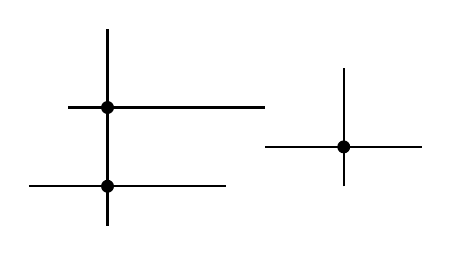
\begin{tikzpicture}[scale=0.5]
\path[draw,thick,-] (0,2) -- (5,2);
\path[draw,thick,-] (1,4) -- (6,4);
\path[draw,thick,-] (6,3) -- (10,3);
\path[draw,thick,-] (2,1) -- (2,6);
\path[draw,thick,-] (8,2) -- (8,5);

\draw[fill] (2,2) circle [radius=0.15];
\draw[fill] (2,4) circle [radius=0.15];
\draw[fill] (8,3) circle [radius=0.15];

\end{tikzpicture}
\end{center}

És fàcil resoldre el problema en temps $O(n^2)$, perquè podem recórrer
tots els parells possibles de segments i comprovar si es
tallen. Tanmateix, podem resoldre el problema de manera més eficient
en temps $O(n \log n)$ fent servir un algorisme de línia d'escombrat i
una estructura de dades de consulta d'interval.

La idea és processar els punts finals dels segments de línia
d'esquerra a dreta i centrar-se en tres tipus d'esdeveniments:
\begin{enumerate}[noitemsep]
\item[(1)] comença un segment horitzontal
\item[(2)] un segment horitzontal acaba
\item[(3)] apareix un segment vertical
\end{enumerate}

Els esdeveniments següents corresponen a l'exemple:
\begin{center}
\begin{tikzpicture}[scale=0.6]
\path[draw,dashed] (0,2) -- (5,2);
\path[draw,dashed] (1,4) -- (6,4);
\path[draw,dashed] (6,3) -- (10,3);
\path[draw,dashed] (2,1) -- (2,6);
\path[draw,dashed] (8,2) -- (8,5);

\node at (0,2) {$1$};
\node at (5,2) {$2$};
\node at (1,4) {$1$};
\node at (6,4) {$2$};
\node at (6,3) {$1$};
\node at (10,3) {$2$};

\node at (2,3.5) {$3$};
\node at (8,3.5) {$3$};
\end{tikzpicture}
\end{center}

Repassem els esdeveniments d'esquerra a dreta i fem servir una
estructura de dades que manté un conjunt de coordenades $y$ on hi ha un
segment horitzontal actiu. A l'esdeveniment 1, afegim la coordenada $y$
del segment al conjunt, i a l'esdeveniment 2, eliminem la coordenada $y$
del conjunt.

Els punts d'intersecció es calculen a l'esdeveniment 3. Quan hi ha un
segment vertical entre els punts $y_1$ i $y_2$, comptem el nombre de
segments horitzontals actius la coordenada $y$ dels quals està entre
$y_1$ i $y_2$, i afegim aquest nombre al nombre total de punts
d'intersecció.

Per emmagatzemar les coordenades y dels segments horitzontals, podem
utilitzar un arbre binari indexat o arbre de segments, possiblement
amb compressió d'índex. Quan s'utilitzen aquestes estructures, el
processament de cada esdeveniment requereix temps $O(\log n)$, de
manera que el temps total d'execució de l'algorisme és $O(n \log n)$.

\section{Problema de la parella més propera}

\index{parella més proper}

Donat un conjunt de $n$ punts, el nostre problema és trobar dos punts
la distància euclidiana dels quals sigui mínima. Per exemple, si els
punts són
\begin{center}
\begin{tikzpicture}[scale=0.7]
\draw (0,0)--(12,0)--(12,4)--(0,4)--(0,0);

\draw (1,2) circle [radius=0.1];
\draw (3,1) circle [radius=0.1];
\draw (4,3) circle [radius=0.1];
\draw (5.5,1.5) circle [radius=0.1];
\draw (6,2.5) circle [radius=0.1];
\draw (7,1) circle [radius=0.1];
\draw (9,1.5) circle [radius=0.1];
\draw (10,2) circle [radius=0.1];
\draw (1.5,3.5) circle [radius=0.1];
\draw (1.5,1) circle [radius=0.1];
\draw (2.5,3) circle [radius=0.1];
\draw (4.5,1.5) circle [radius=0.1];
\draw (5.25,0.5) circle [radius=0.1];
\draw (6.5,2) circle [radius=0.1];
\end{tikzpicture}
\end{center}

\begin{samepage}
hauríem de trobar els punts següents:
\begin{center}
\begin{tikzpicture}[scale=0.7]
\draw (0,0)--(12,0)--(12,4)--(0,4)--(0,0);

\draw (1,2) circle [radius=0.1];
\draw (3,1) circle [radius=0.1];
\draw (4,3) circle [radius=0.1];
\draw (5.5,1.5) circle [radius=0.1];
\draw[fill] (6,2.5) circle [radius=0.1];
\draw (7,1) circle [radius=0.1];
\draw (9,1.5) circle [radius=0.1];
\draw (10,2) circle [radius=0.1];
\draw (1.5,3.5) circle [radius=0.1];
\draw (1.5,1) circle [radius=0.1];
\draw (2.5,3) circle [radius=0.1];
\draw (4.5,1.5) circle [radius=0.1];
\draw (5.25,0.5) circle [radius=0.1];
\draw[fill] (6.5,2) circle [radius=0.1];
\end{tikzpicture}
\end{center}
\end{samepage}

Aquest és un altre exemple d'un problema que es pot resoldre en temps
$O(n \log n)$ fent servir un algorisme de línia d'escombrat\footnote{A
més d'aquest enfocament, també hi ha un algorisme en temps $O(n \log
n)$ de dividir i véncer \cite{sha75} que divideix els punts en dos
conjunts i resol recursivament el problema dels dos
conjunts.}. Recorrem els punts d'esquerra a dreta i mantenim un valor
$d$: la distància mínima entre dos punts vist fins ara. Per a cada punt,
trobem el punt més proper a l'esquerra. Si la distància és inferior a
$d$, és la nova distància mínima i actualitzem el valor de $d$.

Si el punt actual és $(x,y)$ i hi ha un punt a l'esquerra a una
distància inferior a $d$, la coordenada $x$ d'aquest punt ha d'estar
entre $[x-d,x]$ i la coordenada $y$ ha d'estar entre $[y-d,y+d]$. Per
tant, n'hi ha prou amb considerar només els punts que es troben en
aquests intervals, la qual cosa fa que l'algorisme sigui eficient.

Per exemple, a la imatge següent, la regió marcada amb línies
discontínues conté els punts que estan a distància $d$ o inferior del
punt actiu:

\begin{center}
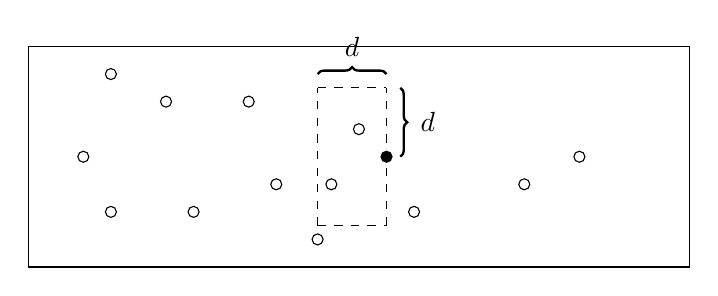
\begin{tikzpicture}[scale=0.7]
\draw (0,0)--(12,0)--(12,4)--(0,4)--(0,0);

\draw (1,2) circle [radius=0.1];
\draw (3,1) circle [radius=0.1];
\draw (4,3) circle [radius=0.1];
\draw (5.5,1.5) circle [radius=0.1];
\draw (6,2.5) circle [radius=0.1];
\draw (7,1) circle [radius=0.1];
\draw (9,1.5) circle [radius=0.1];
\draw (10,2) circle [radius=0.1];
\draw (1.5,3.5) circle [radius=0.1];
\draw (1.5,1) circle [radius=0.1];
\draw (2.5,3) circle [radius=0.1];
\draw (4.5,1.5) circle [radius=0.1];
\draw (5.25,0.5) circle [radius=0.1];
\draw[fill] (6.5,2) circle [radius=0.1];

\draw[dashed] (6.5,0.75)--(6.5,3.25);
\draw[dashed] (5.25,0.75)--(5.25,3.25);
\draw[dashed] (5.25,0.75)--(6.5,0.75);
\draw[dashed] (5.25,3.25)--(6.5,3.25);

\draw [decoration={brace}, decorate, line width=0.3mm] (5.25,3.5) -- (6.5,3.5);
\node at (5.875,4) {$d$};
\draw [decoration={brace}, decorate, line width=0.3mm] (6.75,3.25) -- (6.75,2);
\node at (7.25,2.625) {$d$};
\end{tikzpicture}
\end{center}

L'eficiència de l'algorisme es basa en el fet que la regió sempre
conté només $O(1)$ punts\footnote{(N. del T.) Això és degut que la
regió marcada amb línies discontínues té alçada $2d$, i tots els punts
vistos fins ara estan a distància $d$ o superior.}. Podem recórrer
aquests punts en temps $O(\log n)$ mantenint un conjunt de punts la
coordenada $x$ dels quals està entre $[x-d,x]$, en ordre creixent
segons les seves coordenades $y$.

La complexitat temporal de l'algorisme és $O(n \log n)$, perquè passem
per $n$ punts i trobem per a cada punt el punt més proper a l'esquerra
en temps $O(\log n)$\footnote{(N. del T.) També hem de treure els
punts d'aquest conjunt ordenat quan $d$ es fa més petita o ens movem
cap a la dreta de $(x,y)$, però això també triga temps $O(\log n)$.}.

\section{Problema de l'envolupant convexa}

L'\key{envolupant convexa} (\emph{convex hull}) és el polígon convex
més petit que conté tots els punts d'un conjunt donat. Un poligon és
convex si un segment de línia entre dos vèrtexs qualsevols del polígon
està completament dintre del polígon.

\begin{samepage}
Per exemple, els punts
\begin{center}
\begin{tikzpicture}[scale=0.7]
\draw (0,0) circle [radius=0.1];
\draw (4,-1) circle [radius=0.1];
\draw (7,1) circle [radius=0.1];
\draw (6,3) circle [radius=0.1];
\draw (2,4) circle [radius=0.1];
\draw (0,2) circle [radius=0.1];

\draw (1,1) circle [radius=0.1];
\draw (2,2) circle [radius=0.1];
\draw (3,2) circle [radius=0.1];
\draw (4,0) circle [radius=0.1];
\draw (4,3) circle [radius=0.1];
\draw (5,2) circle [radius=0.1];
\draw (6,1) circle [radius=0.1];
\end{tikzpicture}
\end{center}
\end{samepage}
tenen la següent envolupant convexa:
\begin{center}
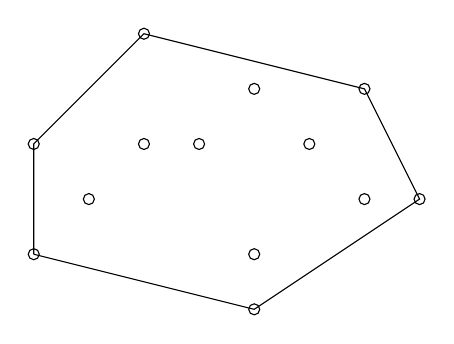
\begin{tikzpicture}[scale=0.7]
\draw (0,0)--(4,-1)--(7,1)--(6,3)--(2,4)--(0,2)--(0,0);

\draw (0,0) circle [radius=0.1];
\draw (4,-1) circle [radius=0.1];
\draw (7,1) circle [radius=0.1];
\draw (6,3) circle [radius=0.1];
\draw (2,4) circle [radius=0.1];
\draw (0,2) circle [radius=0.1];

\draw (1,1) circle [radius=0.1];
\draw (2,2) circle [radius=0.1];
\draw (3,2) circle [radius=0.1];
\draw (4,0) circle [radius=0.1];
\draw (4,3) circle [radius=0.1];
\draw (5,2) circle [radius=0.1];
\draw (6,1) circle [radius=0.1];
\end{tikzpicture}
\end{center}


\index{Algorisme d'Andrew}

\key{L'algorisme d'Andrew} \cite{and79} proporciona una manera
senzilla de construir l'envolupant convexa d'un conjunt de punts en
temps $O(n \log n)$. L'algoritme localitza primer els punts més a
l'esquerra i més a la dreta, i després construeix l'envolupant convexa
en dues parts: primer la part superior i després la part inferior. Les
dues parts són semblants, de manera que ens podem centrar a construir
la part superior.

En primer lloc, ordenem els punts segons la coordenada $x$ i, en cas
d'empat, segons la coordenada $y$. Després d'això, recorrem els punts
i els afegim un a un a l'envolupant convexa, però sempre que n'afegim
un, ens assegurem que l'últim segment de línia de l'envolupant no giri
a l'esquerra. Sempre que giri a l'esquerra treiem repetidament el
penúltim punt de l'envolupant.

Les imatges següents mostren com funciona l'algorisme d'Andrew: \\
\begin{tabular}{ccccccc}
\\
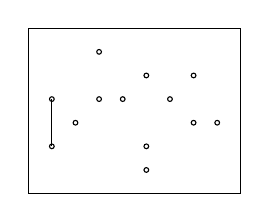
\begin{tikzpicture}[scale=0.3]
\draw (-1,-2)--(8,-2)--(8,5)--(-1,5)--(-1,-2);
\draw (0,0) circle [radius=0.1];
\draw (4,-1) circle [radius=0.1];
\draw (7,1) circle [radius=0.1];
\draw (6,3) circle [radius=0.1];
\draw (2,4) circle [radius=0.1];
\draw (0,2) circle [radius=0.1];

\draw (1,1) circle [radius=0.1];
\draw (2,2) circle [radius=0.1];
\draw (3,2) circle [radius=0.1];
\draw (4,0) circle [radius=0.1];
\draw (4,3) circle [radius=0.1];
\draw (5,2) circle [radius=0.1];
\draw (6,1) circle [radius=0.1];

\draw (0,0)--(0,2);
\end{tikzpicture}
& \hspace{0.1cm} &
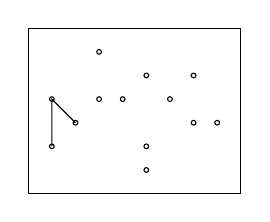
\begin{tikzpicture}[scale=0.3]
\draw (-1,-2)--(8,-2)--(8,5)--(-1,5)--(-1,-2);
\draw (0,0) circle [radius=0.1];
\draw (4,-1) circle [radius=0.1];
\draw (7,1) circle [radius=0.1];
\draw (6,3) circle [radius=0.1];
\draw (2,4) circle [radius=0.1];
\draw (0,2) circle [radius=0.1];

\draw (1,1) circle [radius=0.1];
\draw (2,2) circle [radius=0.1];
\draw (3,2) circle [radius=0.1];
\draw (4,0) circle [radius=0.1];
\draw (4,3) circle [radius=0.1];
\draw (5,2) circle [radius=0.1];
\draw (6,1) circle [radius=0.1];

\draw (0,0)--(0,2)--(1,1);
\end{tikzpicture}
& \hspace{0.1cm} &
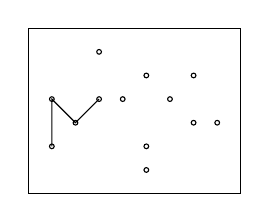
\begin{tikzpicture}[scale=0.3]
\draw (-1,-2)--(8,-2)--(8,5)--(-1,5)--(-1,-2);
\draw (0,0) circle [radius=0.1];
\draw (4,-1) circle [radius=0.1];
\draw (7,1) circle [radius=0.1];
\draw (6,3) circle [radius=0.1];
\draw (2,4) circle [radius=0.1];
\draw (0,2) circle [radius=0.1];

\draw (1,1) circle [radius=0.1];
\draw (2,2) circle [radius=0.1];
\draw (3,2) circle [radius=0.1];
\draw (4,0) circle [radius=0.1];
\draw (4,3) circle [radius=0.1];
\draw (5,2) circle [radius=0.1];
\draw (6,1) circle [radius=0.1];

\draw (0,0)--(0,2)--(1,1)--(2,2);
\end{tikzpicture}
& \hspace{0.1cm} &
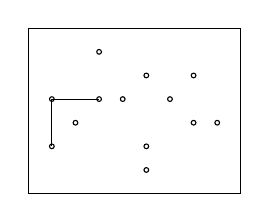
\begin{tikzpicture}[scale=0.3]
\draw (-1,-2)--(8,-2)--(8,5)--(-1,5)--(-1,-2);
\draw (0,0) circle [radius=0.1];
\draw (4,-1) circle [radius=0.1];
\draw (7,1) circle [radius=0.1];
\draw (6,3) circle [radius=0.1];
\draw (2,4) circle [radius=0.1];
\draw (0,2) circle [radius=0.1];

\draw (1,1) circle [radius=0.1];
\draw (2,2) circle [radius=0.1];
\draw (3,2) circle [radius=0.1];
\draw (4,0) circle [radius=0.1];
\draw (4,3) circle [radius=0.1];
\draw (5,2) circle [radius=0.1];
\draw (6,1) circle [radius=0.1];

\draw (0,0)--(0,2)--(2,2);
\end{tikzpicture}
\\
1 & & 2 & & 3 & & 4 \\
\end{tabular}
\\
\begin{tabular}{ccccccc}
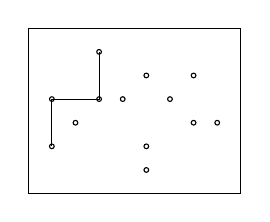
\begin{tikzpicture}[scale=0.3]
\draw (-1,-2)--(8,-2)--(8,5)--(-1,5)--(-1,-2);
\draw (0,0) circle [radius=0.1];
\draw (4,-1) circle [radius=0.1];
\draw (7,1) circle [radius=0.1];
\draw (6,3) circle [radius=0.1];
\draw (2,4) circle [radius=0.1];
\draw (0,2) circle [radius=0.1];

\draw (1,1) circle [radius=0.1];
\draw (2,2) circle [radius=0.1];
\draw (3,2) circle [radius=0.1];
\draw (4,0) circle [radius=0.1];
\draw (4,3) circle [radius=0.1];
\draw (5,2) circle [radius=0.1];
\draw (6,1) circle [radius=0.1];

\draw (0,0)--(0,2)--(2,2)--(2,4);
\end{tikzpicture}
& \hspace{0.1cm} &
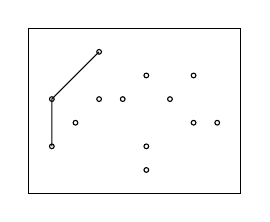
\begin{tikzpicture}[scale=0.3]
\draw (-1,-2)--(8,-2)--(8,5)--(-1,5)--(-1,-2);
\draw (0,0) circle [radius=0.1];
\draw (4,-1) circle [radius=0.1];
\draw (7,1) circle [radius=0.1];
\draw (6,3) circle [radius=0.1];
\draw (2,4) circle [radius=0.1];
\draw (0,2) circle [radius=0.1];

\draw (1,1) circle [radius=0.1];
\draw (2,2) circle [radius=0.1];
\draw (3,2) circle [radius=0.1];
\draw (4,0) circle [radius=0.1];
\draw (4,3) circle [radius=0.1];
\draw (5,2) circle [radius=0.1];
\draw (6,1) circle [radius=0.1];

\draw (0,0)--(0,2)--(2,4);
\end{tikzpicture}
& \hspace{0.1cm} &
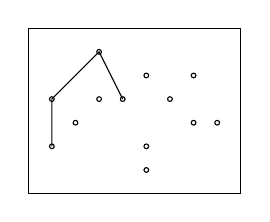
\begin{tikzpicture}[scale=0.3]
\draw (-1,-2)--(8,-2)--(8,5)--(-1,5)--(-1,-2);
\draw (0,0) circle [radius=0.1];
\draw (4,-1) circle [radius=0.1];
\draw (7,1) circle [radius=0.1];
\draw (6,3) circle [radius=0.1];
\draw (2,4) circle [radius=0.1];
\draw (0,2) circle [radius=0.1];

\draw (1,1) circle [radius=0.1];
\draw (2,2) circle [radius=0.1];
\draw (3,2) circle [radius=0.1];
\draw (4,0) circle [radius=0.1];
\draw (4,3) circle [radius=0.1];
\draw (5,2) circle [radius=0.1];
\draw (6,1) circle [radius=0.1];

\draw (0,0)--(0,2)--(2,4)--(3,2);
\end{tikzpicture}
& \hspace{0.1cm} &
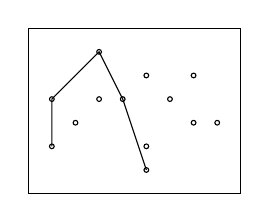
\begin{tikzpicture}[scale=0.3]
\draw (-1,-2)--(8,-2)--(8,5)--(-1,5)--(-1,-2);
\draw (0,0) circle [radius=0.1];
\draw (4,-1) circle [radius=0.1];
\draw (7,1) circle [radius=0.1];
\draw (6,3) circle [radius=0.1];
\draw (2,4) circle [radius=0.1];
\draw (0,2) circle [radius=0.1];

\draw (1,1) circle [radius=0.1];
\draw (2,2) circle [radius=0.1];
\draw (3,2) circle [radius=0.1];
\draw (4,0) circle [radius=0.1];
\draw (4,3) circle [radius=0.1];
\draw (5,2) circle [radius=0.1];
\draw (6,1) circle [radius=0.1];

\draw (0,0)--(0,2)--(2,4)--(3,2)--(4,-1);
\end{tikzpicture}
\\
5 & & 6 & & 7 & & 8 \\
\end{tabular}
\\
\begin{tabular}{ccccccc}
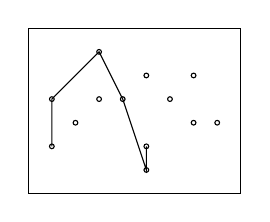
\begin{tikzpicture}[scale=0.3]
\draw (-1,-2)--(8,-2)--(8,5)--(-1,5)--(-1,-2);
\draw (0,0) circle [radius=0.1];
\draw (4,-1) circle [radius=0.1];
\draw (7,1) circle [radius=0.1];
\draw (6,3) circle [radius=0.1];
\draw (2,4) circle [radius=0.1];
\draw (0,2) circle [radius=0.1];

\draw (1,1) circle [radius=0.1];
\draw (2,2) circle [radius=0.1];
\draw (3,2) circle [radius=0.1];
\draw (4,0) circle [radius=0.1];
\draw (4,3) circle [radius=0.1];
\draw (5,2) circle [radius=0.1];
\draw (6,1) circle [radius=0.1];

\draw (0,0)--(0,2)--(2,4)--(3,2)--(4,-1)--(4,0);
\end{tikzpicture}
& \hspace{0.1cm} &
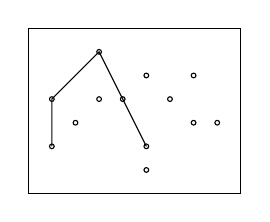
\begin{tikzpicture}[scale=0.3]
\draw (-1,-2)--(8,-2)--(8,5)--(-1,5)--(-1,-2);
\draw (0,0) circle [radius=0.1];
\draw (4,-1) circle [radius=0.1];
\draw (7,1) circle [radius=0.1];
\draw (6,3) circle [radius=0.1];
\draw (2,4) circle [radius=0.1];
\draw (0,2) circle [radius=0.1];

\draw (1,1) circle [radius=0.1];
\draw (2,2) circle [radius=0.1];
\draw (3,2) circle [radius=0.1];
\draw (4,0) circle [radius=0.1];
\draw (4,3) circle [radius=0.1];
\draw (5,2) circle [radius=0.1];
\draw (6,1) circle [radius=0.1];

\draw (0,0)--(0,2)--(2,4)--(3,2)--(4,0);
\end{tikzpicture}
& \hspace{0.1cm} &
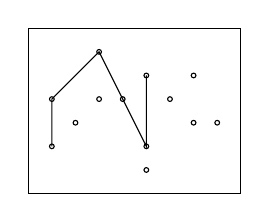
\begin{tikzpicture}[scale=0.3]
\draw (-1,-2)--(8,-2)--(8,5)--(-1,5)--(-1,-2);
\draw (0,0) circle [radius=0.1];
\draw (4,-1) circle [radius=0.1];
\draw (7,1) circle [radius=0.1];
\draw (6,3) circle [radius=0.1];
\draw (2,4) circle [radius=0.1];
\draw (0,2) circle [radius=0.1];

\draw (1,1) circle [radius=0.1];
\draw (2,2) circle [radius=0.1];
\draw (3,2) circle [radius=0.1];
\draw (4,0) circle [radius=0.1];
\draw (4,3) circle [radius=0.1];
\draw (5,2) circle [radius=0.1];
\draw (6,1) circle [radius=0.1];

\draw (0,0)--(0,2)--(2,4)--(3,2)--(4,0)--(4,3);
\end{tikzpicture}
& \hspace{0.1cm} &
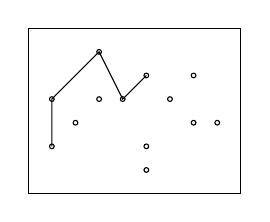
\begin{tikzpicture}[scale=0.3]
\draw (-1,-2)--(8,-2)--(8,5)--(-1,5)--(-1,-2);
\draw (0,0) circle [radius=0.1];
\draw (4,-1) circle [radius=0.1];
\draw (7,1) circle [radius=0.1];
\draw (6,3) circle [radius=0.1];
\draw (2,4) circle [radius=0.1];
\draw (0,2) circle [radius=0.1];

\draw (1,1) circle [radius=0.1];
\draw (2,2) circle [radius=0.1];
\draw (3,2) circle [radius=0.1];
\draw (4,0) circle [radius=0.1];
\draw (4,3) circle [radius=0.1];
\draw (5,2) circle [radius=0.1];
\draw (6,1) circle [radius=0.1];

\draw (0,0)--(0,2)--(2,4)--(3,2)--(4,3);
\end{tikzpicture}
\\
9 & & 10 & & 11 & & 12 \\
\end{tabular}
\\
\begin{tabular}{ccccccc}
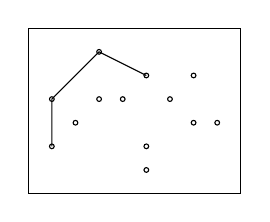
\begin{tikzpicture}[scale=0.3]
\draw (-1,-2)--(8,-2)--(8,5)--(-1,5)--(-1,-2);
\draw (0,0) circle [radius=0.1];
\draw (4,-1) circle [radius=0.1];
\draw (7,1) circle [radius=0.1];
\draw (6,3) circle [radius=0.1];
\draw (2,4) circle [radius=0.1];
\draw (0,2) circle [radius=0.1];

\draw (1,1) circle [radius=0.1];
\draw (2,2) circle [radius=0.1];
\draw (3,2) circle [radius=0.1];
\draw (4,0) circle [radius=0.1];
\draw (4,3) circle [radius=0.1];
\draw (5,2) circle [radius=0.1];
\draw (6,1) circle [radius=0.1];

\draw (0,0)--(0,2)--(2,4)--(4,3);
\end{tikzpicture}
& \hspace{0.1cm} &
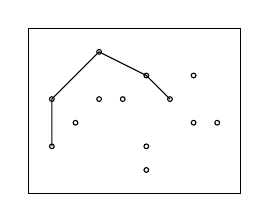
\begin{tikzpicture}[scale=0.3]
\draw (-1,-2)--(8,-2)--(8,5)--(-1,5)--(-1,-2);
\draw (0,0) circle [radius=0.1];
\draw (4,-1) circle [radius=0.1];
\draw (7,1) circle [radius=0.1];
\draw (6,3) circle [radius=0.1];
\draw (2,4) circle [radius=0.1];
\draw (0,2) circle [radius=0.1];

\draw (1,1) circle [radius=0.1];
\draw (2,2) circle [radius=0.1];
\draw (3,2) circle [radius=0.1];
\draw (4,0) circle [radius=0.1];
\draw (4,3) circle [radius=0.1];
\draw (5,2) circle [radius=0.1];
\draw (6,1) circle [radius=0.1];

\draw (0,0)--(0,2)--(2,4)--(4,3)--(5,2);
\end{tikzpicture}
& \hspace{0.1cm} &
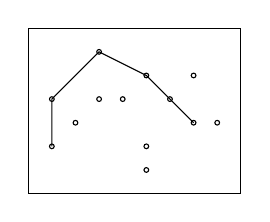
\begin{tikzpicture}[scale=0.3]
\draw (-1,-2)--(8,-2)--(8,5)--(-1,5)--(-1,-2);
\draw (0,0) circle [radius=0.1];
\draw (4,-1) circle [radius=0.1];
\draw (7,1) circle [radius=0.1];
\draw (6,3) circle [radius=0.1];
\draw (2,4) circle [radius=0.1];
\draw (0,2) circle [radius=0.1];

\draw (1,1) circle [radius=0.1];
\draw (2,2) circle [radius=0.1];
\draw (3,2) circle [radius=0.1];
\draw (4,0) circle [radius=0.1];
\draw (4,3) circle [radius=0.1];
\draw (5,2) circle [radius=0.1];
\draw (6,1) circle [radius=0.1];

\draw (0,0)--(0,2)--(2,4)--(4,3)--(5,2)--(6,1);
\end{tikzpicture}
& \hspace{0.1cm} &
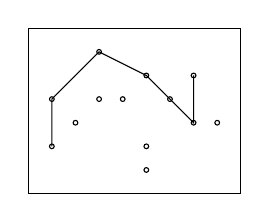
\begin{tikzpicture}[scale=0.3]
\draw (-1,-2)--(8,-2)--(8,5)--(-1,5)--(-1,-2);
\draw (0,0) circle [radius=0.1];
\draw (4,-1) circle [radius=0.1];
\draw (7,1) circle [radius=0.1];
\draw (6,3) circle [radius=0.1];
\draw (2,4) circle [radius=0.1];
\draw (0,2) circle [radius=0.1];

\draw (1,1) circle [radius=0.1];
\draw (2,2) circle [radius=0.1];
\draw (3,2) circle [radius=0.1];
\draw (4,0) circle [radius=0.1];
\draw (4,3) circle [radius=0.1];
\draw (5,2) circle [radius=0.1];
\draw (6,1) circle [radius=0.1];

\draw (0,0)--(0,2)--(2,4)--(4,3)--(5,2)--(6,1)--(6,3);
\end{tikzpicture}
\\
13 & & 14 & & 15 & & 16 \\
\end{tabular}
\\
\begin{tabular}{ccccccc}
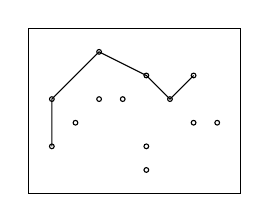
\begin{tikzpicture}[scale=0.3]
\draw (-1,-2)--(8,-2)--(8,5)--(-1,5)--(-1,-2);
\draw (0,0) circle [radius=0.1];
\draw (4,-1) circle [radius=0.1];
\draw (7,1) circle [radius=0.1];
\draw (6,3) circle [radius=0.1];
\draw (2,4) circle [radius=0.1];
\draw (0,2) circle [radius=0.1];

\draw (1,1) circle [radius=0.1];
\draw (2,2) circle [radius=0.1];
\draw (3,2) circle [radius=0.1];
\draw (4,0) circle [radius=0.1];
\draw (4,3) circle [radius=0.1];
\draw (5,2) circle [radius=0.1];
\draw (6,1) circle [radius=0.1];

\draw (0,0)--(0,2)--(2,4)--(4,3)--(5,2)--(6,3);
\end{tikzpicture}
& \hspace{0.1cm} &
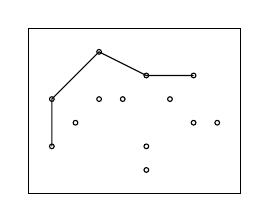
\begin{tikzpicture}[scale=0.3]
\draw (-1,-2)--(8,-2)--(8,5)--(-1,5)--(-1,-2);
\draw (0,0) circle [radius=0.1];
\draw (4,-1) circle [radius=0.1];
\draw (7,1) circle [radius=0.1];
\draw (6,3) circle [radius=0.1];
\draw (2,4) circle [radius=0.1];
\draw (0,2) circle [radius=0.1];

\draw (1,1) circle [radius=0.1];
\draw (2,2) circle [radius=0.1];
\draw (3,2) circle [radius=0.1];
\draw (4,0) circle [radius=0.1];
\draw (4,3) circle [radius=0.1];
\draw (5,2) circle [radius=0.1];
\draw (6,1) circle [radius=0.1];

\draw (0,0)--(0,2)--(2,4)--(4,3)--(6,3);
\end{tikzpicture}
& \hspace{0.1cm} &
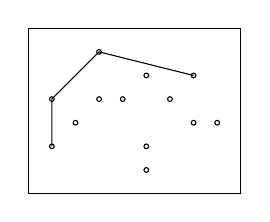
\begin{tikzpicture}[scale=0.3]
\draw (-1,-2)--(8,-2)--(8,5)--(-1,5)--(-1,-2);
\draw (0,0) circle [radius=0.1];
\draw (4,-1) circle [radius=0.1];
\draw (7,1) circle [radius=0.1];
\draw (6,3) circle [radius=0.1];
\draw (2,4) circle [radius=0.1];
\draw (0,2) circle [radius=0.1];

\draw (1,1) circle [radius=0.1];
\draw (2,2) circle [radius=0.1];
\draw (3,2) circle [radius=0.1];
\draw (4,0) circle [radius=0.1];
\draw (4,3) circle [radius=0.1];
\draw (5,2) circle [radius=0.1];
\draw (6,1) circle [radius=0.1];

\draw (0,0)--(0,2)--(2,4)--(6,3);
\end{tikzpicture}
& \hspace{0.1cm} &
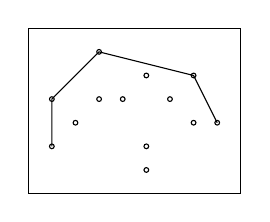
\begin{tikzpicture}[scale=0.3]
\draw (-1,-2)--(8,-2)--(8,5)--(-1,5)--(-1,-2);
\draw (0,0) circle [radius=0.1];
\draw (4,-1) circle [radius=0.1];
\draw (7,1) circle [radius=0.1];
\draw (6,3) circle [radius=0.1];
\draw (2,4) circle [radius=0.1];
\draw (0,2) circle [radius=0.1];

\draw (1,1) circle [radius=0.1];
\draw (2,2) circle [radius=0.1];
\draw (3,2) circle [radius=0.1];
\draw (4,0) circle [radius=0.1];
\draw (4,3) circle [radius=0.1];
\draw (5,2) circle [radius=0.1];
\draw (6,1) circle [radius=0.1];

\draw (0,0)--(0,2)--(2,4)--(6,3)--(7,1);
\end{tikzpicture}
\\
17 & & 18 & & 19 & & 20
\end{tabular}
